\documentclass{article} % Choose class of document

% Define required packages here 
\usepackage{nomencl}
\usepackage[margin=2cm, bottom=3cm]{geometry}
\usepackage[bottom]{footmisc}
\usepackage{setspace}
\usepackage{graphicx}
\usepackage{subcaption}
\usepackage{float}
\usepackage{import}
\usepackage{xcolor}
\usepackage{placeins}
\usepackage{fancyhdr}
\usepackage{titlesec}
\usepackage{amsmath}
\usepackage[justification=centering]{caption}

% Set up fancyhdr for custom headers
\pagestyle{fancy}
\fancyhead[L]{Thesis A} % "thesis" on the left
\fancyhead[R]{Nathan Sivalingam} % Your name on the right
\renewcommand{\headrulewidth}{0pt}
\setlength{\headheight}{30pt}  % Adjust this value for header height (default is 12pt)

% Set the spacing between lines of the document
\onehalfspacing

% Command for nomenclature which is defined here prior to the start of the document
\makenomenclature
\renewcommand{\nompreamble}{(The nomenclature must respect the following order: latin symbols, Greek symbols, acronyms. Within each category of symbols, follow alphabetic order. An example is provided below)}

% The document commences here (everything above is used to set up the .tex file
\begin{document}

% Input the Title Page .tex file here (inputs have been used to collate the section and manage the document easier).
% Define the UNSW logo and title of the thesis here, including author and supervisor names
\title{
    
\includegraphics[width=0.5\textwidth]{Figures/unsw_crest.jpg}\\ \vspace{10mm}
    \textbf{MMAN4951 - UG Thesis A\\ 
    % Investigating the Height and Position Effects of Vortex Generators on the Electrical Efficiency of Photovoltaic Modules under Forced Convection Conditions
    \textit{Interim Report and Project Plan\vspace{6mm}}}
    } 
\author{Author: Nathan Sivalingam, z5359644 \vspace{2mm} \\ Supervisor: Dr Charitha de Silva\vspace{4mm} \\ UNSW Sydney, School of Mechanical \& Manufacturing Engineering}
\date{25/04/2025} % Can include the date of submission here

% Creates the title defined above
\maketitle

% Originality Statement
\pagebreak

% Abstract
% \begin{abstract}
%     Write a short abstract outlining the importance of the project, your progress to date, and your planned future work. Do not exceed 100 words in the abstract. The maximum length of the entire report is 20 pages, excluding appendices. This will form a strong foundation for your final Research Thesis report. Please regard this as a great opportunity to collect your initial thoughts and data. You can use Microsoft Word or other document editors such as LaTeX, InDesign, or OpenOffice, however font sizes and margins should be similar to this guide. NOTE: this guide is indicative and can be modified in agreement with your supervisor. Please refer to the course outline (marking criteria and rubrics) for more details about expectations for each section.
% \end{abstract}

\pagebreak

% Table of Contents
\tableofcontents

\pagebreak

% The nomenclature section is created here (variables and definitions can be edited below).
% \nomenclature[1A]{\(A\)}{amplitude of …}
% \nomenclature[1Cp]{\(C_p\)}{…}
% \nomenclature[1D]{\(D\)}{…}
% \nomenclature[1alpha]{\(\alpha\)}{…}
% \nomenclature[2TLA]{\(TLA\)}{…}

\renewcommand{\nomgroup}[1]{%
  \ifthenelse{\equal{#1}{A}}{\item[\textbf{Abbreviations}]}{}%
  \ifthenelse{\equal{#1}{B}}{\item[\textbf{Parameters}]}{}%
  \ifthenelse{\equal{#1}{C}}{\item[\textbf{Greek Symbols}]}{}%
  \ifthenelse{\equal{#1}{D}}{\item[\textbf{Subscripts}]}{}%
}

\nomenclature[A]{\(PV\)}{photovoltaic}
\nomenclature[A]{\(PIV\)}{particle image velocimetry}
\nomenclature[A]{\(AM\)}{air mass}
\nomenclature[A]{\(MTFHS\)}{multidirectional tapered fin heat sinks}
\nomenclature[A]{\(PCM\)}{phase change materials}
\nomenclature[A]{\(PDMS\)}{polydimethylsiloxane}

% Work Function Equation
\nomenclature[B]{\(E\)}{work function (J)}
\nomenclature[B]{\(h\)}{Planck's constant (J s)}
\nomenclature[B]{\(f_0\)}{threshold frequency (Hz)}

% Electrical Efficiency Equation
\nomenclature[B]{\(\eta\)}{electrical efficiency}
\nomenclature[B]{\(V_\text{OC}\)}{open-circuit voltage (v)}
\nomenclature[B]{\(I_\text{SC}\)}{short-circuit current (A)}
\nomenclature[B]{\(FF\)}{fill factor}
\nomenclature[B]{\(P_\text{in}\)}{power input (W)}

% Minimum Diode Saturation Current Equation
\nomenclature[B]{\(J_0\)}{diode saturation current ($A/m^2$)}
\nomenclature[B]{\(q\)}{elementary charge ($1.602\times10^{-19}$ C)}
\nomenclature[B]{\(k\)}{Boltzmann constant ($1.381\times10^{-23}\;J K^{-1}$)}
\nomenclature[B]{\(\sigma\)}{Stefan-Boltzmann constant ($5.670\times10^{-8}\; W/(m^2K^4$)}
\nomenclature[B]{\(T\)}{temperature (K)}
\nomenclature[B]{\(E_g\)}{band gap (eV)}

% Open-circuit voltage Equation
% \nomenclature[B]{\(n\)}{}
% \nomenclature[B]{\(I_0\)}{}
% \nomenclature[B]{\(I_L\)}{}


\printnomenclature

% The students email is inserted below
\footnotetext[1]{contact email: n.sivalingam@student.unsw.edu.au}


% Page breaks can be used to start a new page
\pagebreak

% Input the Introduction Page .tex file here
\section{Introduction}

THIS document provides a guide for you to use for your Thesis A report. It is also intended to provide you with some structure and to help you understand the standard of writing required for your final submission – take it as an opportunity to get right into the habit of high-quality technical reporting. The style of writing here, including how figures are labeled, how referencing is done, and the general flow of a research report (that will be fleshed out into your thesis), is what is expected of you. You can use this guide fully or just reproduce your own, but font sizes and margins should be similar to this guide. Your report should have a similar tone and style to the peer-reviewed literature that you have already been reading. It is preferred that you speak in the “scientific voice”, i.e. “the humidity was calculated”, rather than “I calculated the humidity”. Keep the language objective, and be specific where you can be; for instance use “significantly altered from the test conditions” and “20\% greater”, rather than “amazingly, it was drastically different from the test conditions” and “a bit more”. % Percentage symbols are used in Latex to make comments so to use a % symbol in text use the above syntax
	\\ % These are used to create a new line
	\\
In this section, you should introduce your topic (to a reader who is an engineer, but may not be fully familiar with your topic – this is for the benefit of readers other than your supervisor, i.e. the moderator or incoming future students). Here you need only reference very significant literature, and provide an overview of what the field is, what your project is, why your project is important, and very briefly how you intend(ed) on going about the work. It should set up the literature review – the reader now knows roughly what they are reading about and what they are looking for in the coming section(s). 
	\\
	\\ % \textbf{} is used to bold the included words
The introduction might run to \textbf{about 1 to 1.5 pages}, assuming a figure or two showing something highly useful for the reader, such as a picture of the problem (perhaps with annotation), and maybe some kind of flowchart showing the workflow. 

\section{Literature Review}
\textit{What is the problem to be solved, and it's significance?
\begin{itemize}
    \item Brief background to project
    \item Summary of literature relevant to project
    \item Identification of "gaps" in the literature
\end{itemize}}

The literature review is not just about presenting descriptions of the important papers you have found, but telling a meaningful story and, where appropriate, some critical discussion of previous findings (i.e. was another study useful but flawed?). Remember that you may read hundreds of papers/books/web pages etc., but often only about 20 or 30 are really important, and these are the ones you will mention in your literature review, which this report will be a concise version of. This section needs to flow logically, and this does not always imply that the material is chronological. By the end, the reader should have a clear appreciation of what the major work in the field was, why it is relevant to the current project, and where the unknowns and questions lie (\textbf{research gaps}) – these are the issues that you are going to address with your thesis research.

For the purposes of this report, this section will be \textbf{12-15 pages long}. Remember to reference properly any material that you obtain from literature or other sources. If you are unsure how to discuss literature properly, find a really good review paper on your topic, or if there isn’t one, a similar topic, and you will have a good example to refer to.

\subsection{Principles of Photovoltaic Modules}
\subsubsection{What are photovoltaic modules?}
Photovoltaic modules, commonly known as solar panels, are devices that convert sunlight into electrical energy.\vspace{0.5em}

\subsubsection{What is the photoelectric effect?}
Sunlight is made up of massless particles called photons which possess a certain amount of energy. When these photons strike the surface, they knock electrons off of it, known as photoelectrons. This is known as the photoelectric effect.\vspace{0.5em}

\noindent The photoelectric effect will occur only if the frequency of the radiation is greater than the threshold frequency of the metal. The threshold frequency is the minimum frequency of light that causes electrons to be emitted from a material. The proportional relationship that exists between the threshold frequency and the work function is shown in equation \ref{eq:workfunction} below:
\begin{equation}
    E = hf_0
    \label{eq:workfunction}
\end{equation}
Where:
\begin{itemize}
    \item $E$ is the work function.
    \item ($h = 6.62607015 \times 10^{34}$ joule-second) is Planck's constant.
    \item $f_0$ is the threshold frequency. 
\end{itemize}\vspace{0.5em}
\noindent The work function refers to the minimum amount of energy needed to remove an electron from a metal surface. If photons with enough energy hit the surface, they can transfer their energy to the electrons allowing them to escape. If the energy of the incident photons is less than the work function, no electrons will be emitted, regardless of the intensity of the light.\vspace{0.5em}

\subsubsection{How do photovoltaic modules work?}
A photovoltaic module is made up of multiple photovoltaic cells, commonly known as solar cells. Each photovoltaic cell is made of semiconductor material. The most common semiconductor material used to make photovoltaic cells is silicon, accounting for 95 percent of photovoltaic modules sold worldwide. These photovoltaic cells use the photovoltaic effect to convert solar energy into electrical energy.\vspace{0.5em}

\noindent A silicon photovoltaic cell is composed of two different layers of silicon, shown below in Figure \ref{fig:photovoltaic_cell_diagram}:

\begin{figure}[h]
    \centering
    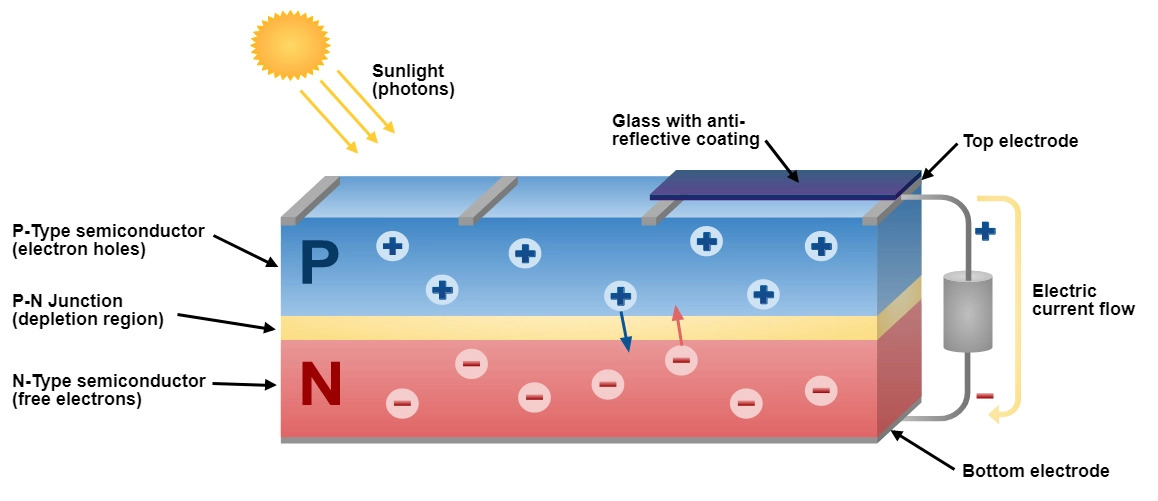
\includegraphics[width=1\textwidth]{Figures/photovoltaic_cell_diagram.jpg}
    \caption{An example figure.}
    \label{fig:photovoltaic_cell_diagram}
\end{figure}

\FloatBarrier

\noindent - In a photovoltaic cell, crystalline silicon is sandwiched between conductive layers.\par
\noindent - Each silicon atom is connected to its neighbours by four strong bonds.\par
\noindent - A silicon photovoltaic cell uses two different layers of silicon.\par
\begin{itemize}
    \item An n-type silicon, which has extra electrons.
    \item A p-type silicon has extra spaces for electrons, called holes.
\end{itemize}
\noindent - Where the two types of silicon meet, electrons can wander across the p/n junction, leaving a positive charge on one side and creating negative charge on the other.\par

\noindent - When a photon strikes the silicon cell with enough energy, it can knock an electron from it's bond, leaving a hole.\par
\noindent - The negatively charged electron and location of the positively charged hole are now free to move around.\par
\noindent - Because of the electric field at the p/n junction, they will only go one way.\par
\noindent - They electron is drawn to the n-side while the hole is drawn to the p-side.\par
\noindent - The mobile electrons are collected by thin metal fingers at the top of the cell.\par
\noindent - From there, they flow through an external circuit, doing electrical work, like powering a light bulb, before returning through the conductive aluminium sheet on the back.\par
\noindent - Each photovoltaic cell only puts out half a volt, but you can string them together in modules to get more power.\par
\noindent - Electrons are the only moving parts in a photovoltaic cell, and the go back to where they came from, so there is nothing to get worn out, or used up.\par
\noindent - Therefore, photovoltaic cells can last for decades.\vspace{0.5em}

\noindent \textit{So what is the reason that photovoltaic modules don't last forever -- Lead into the limitations of photovoltaic modules}






\subsection{Limitations of Photovoltaic Modules}
\begin{itemize}
    \item What are the limitations of photovoltaic modules?
\end{itemize}

\subsection{Heat Transfer in Photovoltaic Modules}
\begin{itemize}
    \item What is heat transfer?
    \item What are the types of heat transfer?
    \item What is the fundamental concept of heat transfer?
    \item What are some convection principles used to enhance heat transfer in a photovoltaic module?
\end{itemize}

\subsubsection{Vortex Induced Heat Transfer}
\begin{itemize}
    \item What is a vortex?
    \item How does a vortex/system of vortexes induce heat transfer?
    \item Are there any drawbacks of vortex-induced heat transfer? If so, what are they?
\end{itemize}

\subsubsection{Conduction}
\begin{itemize}
    \item What is conduction?
    \item How can conduction be used to enhance heat transfer?
    \item What are some examples of this principle in practice?
    \item What were the results of this practice?
    \item Are there any drawbacks of conduction as a method to enhance heat transfer?
\end{itemize}

\subsubsection{Radiation}
\begin{itemize}
    \item What is radiation?
    \item How can radiation be used to enhance heat transfer?
    \item What are some examples of this principle in practice?
    \item What were the results of this practice?
    \item Are there any drawbacks of radiation as a method to enhance heat transfer?
\end{itemize}

\subsection{Convective Photovoltaic Module Cooling Methods}
\begin{itemize}
    \item What is convection?
    \item What are some cooling methods for convective photovoltaic modules?
\end{itemize}

\subsubsection{Cooling through Natural Convection}
\begin{itemize}
    \item What is Natural Convection?
    \item How is natural convection used as a cooling method for photovoltaic modules?
    \item Are there drawbacks to natural convection as a cooling method for photovoltaic modules?
    \item How does forced convection compare to natural convection as a cooling method for photovoltaic modules?
\end{itemize}

\subsubsection{Cooling through Forced Convection}
\begin{itemize}
    \item What is forced convection?
    \item How is forced convection used as a cooling method for photovoltaic modules?
    \begin{itemize}
        \item DC Fan Experiment
        \item Floating Photovoltaic Module Experiment
    \end{itemize}
    \item Are there drawbacks to forced convection as a cooling method for photovoltaic modules?
    \item Air vs Water Cooling Experiment
    \item Air Cooled Modified Photovoltaic Module Experiment
    \item Single Fin vs Multiple Fin Experiment
\end{itemize}

\subsubsection{Cooling through Vortex Generators}
\begin{itemize}
    \item What is a vortex generator?
    \item What is the purpose of vortex generators?
    \item Examples of Vortex Generator Experiments in the Context of Photovoltaic Module Cooling
\end{itemize}
\section{Research Question and Project Plan}

% This section will start with a clear statement on your research question, i.e. what you want to discover in relation to the already available literature and its gaps (connect to previous section). Hypothesis and aims at the basis of your research will also be presented to detail your research question, again in relation to what has been already observed in literature (e.g. a particular aspect is not considered because multiple studies have shown it is not relevant). After detailing your research question, you will describe with technical detail how you are going to conduct your research (research plan). In particular you should discuss:

% Use itemize to create dot points
\subsection{Research Question}
\subsection{Hypothesis and Aims}
\pagebreak

\subsection{Proposed Solution/Experimental Methodology}
\pagebreak

\subsection{Thesis timeline - for next two terms}
\subsubsection{Term 2, 2025}
\noindent \textbf{Justification of Time Allocation}
\pagebreak

\subsubsection{Term 3, 2025}
\noindent \textbf{Justification of Time Allocation}
\pagebreak

\subsection{Available Resources}
\subsection{Required Training and Upskilling}
\begin{itemize}
    \item your proposed solution/experimental methodology to address the research question;
    \item your thesis timeline (possibly with a Gantt chart or some kind of dated mindmap, which can go in appendix, and can be referenced to in this section) and a justification of time allocation for each task;
    \begin{itemize}
        \item Two Gantt charts, see if you are allowed to create them on landscape A4 templates
        \item Add a justification for each time allocation
        \item Create affordable delay periods and explain why you included that as well (Check MECH4100's feedback on your Gantt chart to ensure that it is perfect)
    \end{itemize}
    \item the resources you have identified as available to your research; and
    \begin{itemize}
        \item UNSW Past Research Papers (Sophie, Ishan, Ziao Zhou, Matt's RIR, the Published Report with Svetlana)
        \item Research Papers published by other Universities (Add them here as you find them)
        \item Human resources that are currently working on the project/can help in the Aero Lab (Charitha de Silva, Matthew Deng, Shubneet Sodhi, Mark Zhai)
        \item Books that I may need to check out of the UNSW library (add them here as you go)
        \item Online tools/software (MATLAB, FLIR, Overleaf, Excel, Teams, Outlook, Mendeley)
        \item Physical Locations (Aero Lab, ENG Maker-space, UNSW Library)
    \end{itemize}
    \item the required training and upskilling that you will need to obtain.
    \begin{itemize}
        \item Aero Lab Induction (All Online Training Modules, Physical Induction from Mark Zhai)
        \item Aero Lab Tour (Physical Induction by Matthew Deng)
        \item Maker-space Induction (Workshop Safety Badge (includes Online Module, Quiz and a Physical Induction) - YET TO DO
        \item MATLAB Induction (From Matthew Deng) - COMPLETED BUT THERE IS NO OFFICIAL CERTIFICATE, SO PERHAPS AN ACKNOWLEDGEMENT WILL BE FINE
        \item Online MATLAB Tutorials/Workshops because it is a big part of the project - YET TO DO
        \item Online FLIR tutorials/workshops because it is how the data is processed - YET TO DO
    \end{itemize}
\end{itemize}
Try to correlate textual descriptions with visual aids (e.g. pictures of your experimental rig).
This section is \textbf{3-5 pages} long. 

\pagebreak
\section{Project Dependent Preparations}

\subsection{Evidence of training on specific equipment and/or up-skilling in new software methods}
\noindent \textbf{Wind Tunnel}\par
\noindent \textbf{MATLAB}\par
\noindent \textbf{Flir}\par

\subsection{Preliminary results/sketches}
\noindent \textbf{Aligned on Roof: 20 mm Vortex Generators (1 m/s, 2 m/s, 3 m/s)}\par
\noindent \textbf{Aligned on Roof: 75 mm Vortex Generators (1 m/s, 2 m/s, 3 m/s)}\par
\noindent \textbf{Aligned on Roof: 150 mm Vortex Generators (1 m/s, 2 m/s, 3 m/s)}\par
% In terms of preliminary results, you are encouraged to present your findings with graphical aids (figures, see example below).

\subsection{Components/parts ordered}
\noindent \textbf{3D Printed Vortex Generators (75 mm)}\par

\subsection{Detailed budget of parts to be ordered}\par
\noindent \textbf{3D Printed Vortex Generators (150 mm)}\par

% The risk management form from mech4100 is in additional reasources. Use it as a guide for this section.
\subsection{Risk Assessment}
\begin{table}[ht]
    \centering
    \caption{Risk Assessment Table}
    \resizebox{\textwidth}{!}{ % Scale the table to the width of the page
        \begin{tabular}{|c|c|c|c|c|c|c|c|}
            \hline
            Task / Scenario & Hazard & Associated Harm & Existing Controls & Additional Controls Required? & Risk Rating & Cost of Controls (Time, Effort, Money) & Reasonable Practice (Y/N) \\ 
            \hline
            % Example Row (Replace with actual data)
            Example Task & Example Hazard & Example Harm & Existing Control & Additional Control & High & Medium & Y \\
            \hline
        \end{tabular}
    }
    \label{tab:my_label}
\end{table}

\pagebreak


% This section will describe, in \textbf{1-2 pages}, your preparations, progress and preliminary results (assuming you have relatively few at this stage). This section should include:

%%%%%%%%%%%%%%%%%%%%%%%%%%%%%%%%%%%%%%%%%%%%%%%%%%%%%%%%%%%%%%%%%%%%%%%%%%%%%%%%%%%%%%%
%%     UNCOMMENT EVERYTHING BELOW AND MAKE SURE YOUR REPORT OBEYS ALL THE RULES
%%     DO IT AT THE END THOUGH, HOPEFULLY EVERYTHING SHOULD BE SWEET
%%%%%%%%%%%%%%%%%%%%%%%%%%%%%%%%%%%%%%%%%%%%%%%%%%%%%%%%%%%%%%%%%%%%%%%%%%%%%%%%%%%%%%%
% %Figures can be created as shown below
% \begin{figure}[H] % [H] positions the figure "here". For more information of positioning of Figure see: https://www.overleaf.com/learn/latex/Positioning_of_Figures and inserting an image here: https://www.overleaf.com/learn/latex/Inserting_Images
%     \centering %Centres the figure in the middle of the page
%     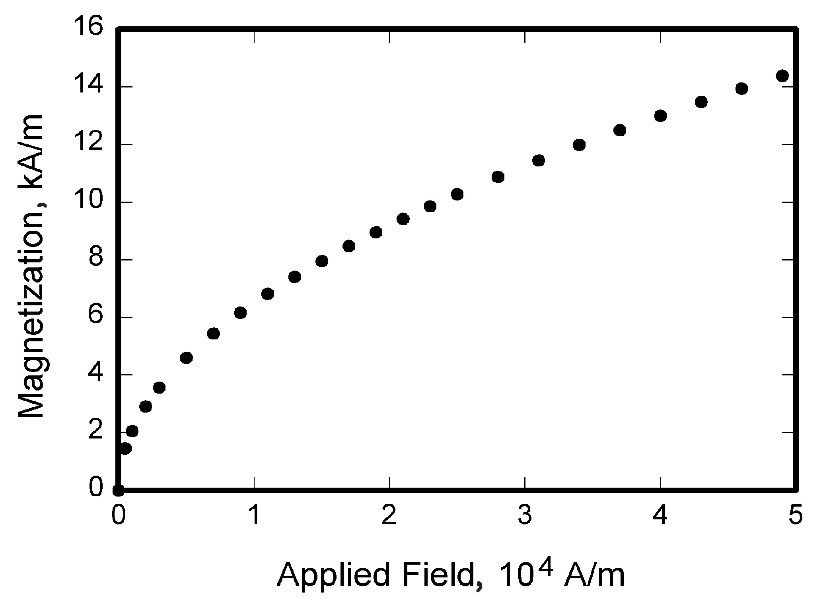
\includegraphics[width=10cm]{Figures/Image 1.jpg} % inserts the figure from the Figures folder (note figures need to be uploaded before inserting).
%     \textbf{\caption{Magnetization as a function of applied field. \normalfont{\textit{Figure captions should be bold and justified, with a period and a single tab (no hyphen or other character) between the figure number and the figure description. If you took a figure from another paper or the web (when permitted), you MUST include a reference in the caption)}}}} %Captions can be included using \caption
% \end{figure}

% \begin{figure}[H]
%     \begin{center} % Another option to centre the figure
%         \subcaption[Dog] % If multiple images are required in a figure, the sub caption option can be used 
%         {
\includegraphics[width=0.24\textwidth]{Figures/Dog.jpg}} % The first image is include with size defined
%         \subcaption[Doge] % Name of the subcaption is defined here
%         {
\includegraphics[width=0.24\textwidth]{Figures/Dog 2.jpg}} % The second image is include with size defined
%         \textbf{\caption{Some Dogs}} % The overall figure caption is defined here
%     \end{center}
% \end{figure} 

% % Tables can be created as shown. Tables can be generated with Latex syntax here: https://www.tablesgenerator.com/ 
% % More information on creating tables can be found here:https://www.overleaf.com/learn/latex/tables
% \begin{table}[H]
%     \textbf{\caption{A Table}} %Table captions are placed above the table
%     \begin{center} % Centres the table
%     \begin{tabular}{ |c|c|c| } 
%     \hline
%     1 & 2 & 3 \\ 
%     4 & 5 & 6 \\ 
%      7 & 8 & 9 \\ 
%     \hline
%     \end{tabular}
%     \end{center} 
% \end{table}

% Tables and figures of all types can be added inline or with text wrapping frames. Place figure captions below all figures; place table titles above the tables. If your figure has multiple parts, include the labels “a),” “b),” etc. below and to the left of each part, above the figure caption. Please verify that the figures and tables you mention in the text actually exist. 

% When citing a figure in the text, use the abbreviation “Fig.” except at the beginning of a sentence. Do not abbreviate “Table.” Number each different type of illustration (i.e., figures, tables, images) sequentially with relation to other illustrations of the same type.

% Figure axis labels are often a source of confusion. Use words rather than symbols. As in the example in Fig. 1, write the quantity “Magnetization” rather than just “M.” Do not enclose units in parenthesis, but rather separate them from the preceding text by commas. Do not label axes only with units. As in Fig. 1, for example, write “Magnetization, A/m” or “Magnetization, $Am^{-1}$,” not just “A/m.” Do not label axes with a ratio of quantities and units. For example, write “Temperature, K,” not “Temperature/K.”

% Equations are centered and numbered consecutively, with equation numbers in parentheses flush right, as in Eq. (1). 

% % Equations are defined as shown below
% \begin{equation}
%     \label{simple_equation} % Labels can be used to cross reference. For more information see: https://www.overleaf.com/learn/latex/Cross%20referencing%20sections,%20equations%20and%20floats
%     Re = \frac{\rho\,UL}{\beta} % Equation is written here
% \end{equation}

% Be sure that the symbols in your equation are defined before the equation appears, or immediately following. Italicize symbols (T might refer to temperature, but T is the unit tesla). Refer to “Eq. (1),” not “(1)” or “equation (1)” except at the beginning of a sentence: “Equation (1) is…” Equations can be labeled other than “Eq.” should they represent inequalities, matrices, or boundary conditions. If what is represented is really more than one equation, the abbreviation “Eqs.” can be used.

% Define abbreviations and acronyms the first time they are used in the text, even after they have already been defined in the abstract. Very common abbreviations such as CFD, SI, ac, and dc do not have to be defined. Abbreviations that incorporate periods should not have spaces: write “P.R.,” not “P. R.” 
\section{Conclusion}

Although a conclusion may review the main points of the work to date, do not simply replicate the abstract. \textbf{Half a page} should be sufficient to concisely summarise everything that’s been done to date.
\section*{Acknowledgments}

Feel free to briefly thank anyone that’s been helping you with your project – lab officer, the workshop, industrial partner, a friend that helped you solve a killer problem – this is a common courtesy in technical writing.

\pagebreak
\bibliographystyle{plain}
\bibliography{Sections/References}
\pagebreak
\section*{Appendix}

Add in the appendices any material which supports this document, but does not “fit” naturally in the flow of your report’s narrative.

Place here your Gantt chart with detailed activities (to be referred to in the project plan section). Feel free to put it in “sideways” to fit better. In the appendix, the more detail the better – make realistic dates and specific milestones, you should have a good idea by now what you need to do and how you’re going to do it... if not, you definitely need to discuss with your supervisor as soon as possible.

Also remember to add your draft thesis outline in the appendices. This is in the form of a table of contents of the Thesis, with detailed sub-section headings linked to your research topic and planned activities.

\begin{itemize}
    \item Equations: Go through all the equations that you mention in your report and explain them in detail (I.e., The formula, what all the variables represent, any additional content required)
\end{itemize}
\end{document}


 